\documentclass[12pt]{article}
\usepackage[utf8]{inputenc}
\usepackage{amsmath,amssymb,latexsym}
\usepackage{enumerate}
\usepackage{graphicx}
\usepackage{float}
\usepackage[spanish]{babel}
\usepackage{xypic}

\textheight=25cm \textwidth=18cm \topmargin=-2cm \oddsidemargin=-1cm

\newcommand{\abs}[1]{\left\vert#1\right\vert}
\newcommand{\norm}[1]{\left\Vert#1\right\Vert}

\newcommand{\Ll}{\mathfrak L}
\newcommand{\R}{\mathbb R}
\newcommand{\x}{\mathrm x}
\newcommand{\To}{\longrightarrow}

\begin{document}

\pagestyle{empty}
\begin{center}
{\textsc{Cálculo Diferencial e Integral III} \\
\medskip 
\large{Ejercicios II - 1 \\
Luis David Uicab Martínez \\
(Derivada de funciones entre espacios euclidianos)}}
\end{center}
\bigskip

\begin{enumerate}

\item Denotemos por $\Ll\subset \R^3$ a la l\'inea recta determinada por la intersecci\'on de los planos $ax+by+cz+d=0$ y $a'x+b'y+c'z+d'=0$. Muestra que: 
\begin{enumerate}[(1)]
\item Si $\x_0=(x_0,y_0,z_0)$ y $\x_1=(x_1,y_1,z_1)$ son dos puntos diferentes que pertenecen a $\Ll$ entonces la aplicaci\'on $\gamma:\R\To \R^3$ dada por 
$\gamma(t)=\x_0+t(\x_1-\x_0)$ es una parametrizaci\'on de $\Ll$.  
\item Si $\x_0\in \Ll$ y $\mathrm u=(u_1,u_2,u_3)\neq 0$ es un vector paralelo a la l\'inea $\Ll$ (i.e., $au_1+bu_2+cu_3=0$ y $a'u_1+b'u_2+c'u_3=0$) entonces la aplicaci\'on $\gamma:\R\To \R^3$ dada por $\gamma(t)=\x_0+t\mathrm u$ es una parametrizaci\'on de $\Ll$.  
\end{enumerate}
\textbf{Demostración.}
\begin{enumerate}[(i)]
    \item Tomemos $t\in \R$ arbitrario. Notemos que, como $\x_0,\x_1 \in \mathcal{L}$, se cumple que
        \begin{align*}
            ax_0+by_0+cz_0+d=0=ax_1+by_1+cz_1+d.
        \end{align*}
        Por otra parte,
        \begin{align*}
            \gamma(t) &= \x_0+t(\x_1-\x_0) \\
            &= (x_0,y_0,z_0) + t((x_1,y_1,z_1)-(x_0,y_0,z_0)) \\
            &= (x_0 + tx_1 -tx_0,y_0 + ty_1 -ty_0,z_0 + tz_1 -tz_0).
        \end{align*}
        Luego, de las igualdades antes mencionadas
        \begin{align*}
            a(x_0 + tx_1 -tx_0)+b(y_0 + ty_1 -ty_0)+c(z_0 + tz_1 -tz_0) + d =& (ax_0+by_0+cz_0 + d) \\
            &+t(ax_1+by_1+cz_1+d) \\
            &-t(ax_0+by_0+cz_0+d) \\ 
            =&0.
        \end{align*}
        De forma análoga, se prueba que $\gamma(t)$ satisface $a'x+b'y+c'z+d'=0$. En consecuencia, $\gamma(t) \in \mathcal{L}$. Por otra parte, dado que $\x_0,\x_1 \in \mathcal{L}$, afirmamos que podemos expresar todo punto $\x$ en $\mathcal{L}$ como
        $\x=\x_0+t(\x_1-\x_0)$. Luego, de dicha definición de $\x$, afirmamos que existe $t_0$ tal que $\x=\gamma(t_0)$. Así, $\x \in \gamma(t)$, de lo que se sigue $\mathcal{L}=\gamma(t)$.

    \item Sea $t$ arbitrario. Tenemos que $\gamma(t)=(x_0,y_0,z_0)+t(u_1,u_2,u_3)=(x_0+tu_1,y_0+tu_2,z_0+tu_3)$. Teniendo en cuenta las igualdades que satisfacen $\x_0$ y $\mathrm u$, obtenemos que
        \begin{align*}
            a(x_0tu_1) + b(y_0+tu_2) + c(z_0+tu_3) + d &= (ax_0 + by_0 + cz_0 + d) + t(au_1+bu_2+cu_3)\\
            &=0.
        \end{align*}
        De forma análoga, se sigue que $\gamma(t)$ es un punto en el plano $a'x+b'y+c'z+d=0$. De ello, tenemos que $\gamma(t)$ está en la intersección de los planos previamente mencionados, y por lo tanto,
        es un punto de $\mathcal{L}$, y por lo tanto, $\gamma$ es una parametrización de dicha recta. \hfill $\blacksquare$
\end{enumerate}

\newpage
\item Determina si las curvas $\Gamma$ con parametrización dada 
$\gamma:(\pi,\infty)\To \R^2$ son regulares y bosqueja sus gráficas:
\begin{enumerate}[(1)]
\item $\gamma(t) = \left( \frac{\cos(t)}{t},\frac{\sen(t)}{t} \right)$.
\item $\gamma(t) = \left( \frac{t+\pi}{t}\cos(t),\frac{t+\pi}{t}\sen(t) \right)$.
\end{enumerate}
\textbf{Solución.}
\begin{enumerate}
    \item Notemos que
    \begin{align*}
        \gamma'(t)=0 &\implies \left(-\frac{\cos(t)}{t^2}-\frac{\sin(t)}{t},-\frac{\sin(t)}{t^2}+\frac{\cos(t)}{t}\right)=\left(0,0\right) \\
        &\implies \left(\frac{-\cos(t)-t\sin(t)}{t^2},\frac{-\sin(t)+t\cos(t)}{t^2}\right)=\left(0,0\right) \\
        &\implies -\cos(t)-t\sin(t)=0, \quad -\sin(t)+t\cos(t)=0 \\
        &\implies \cos(t)=-t\sin(t),  \quad t\cos(t)=\sin(t) \\
        &\implies -t^2\sin(t)=\sin(t) \\
        &\implies t^2\sin(t)+\sin(t)=0 \\
        &\implies \sin(t)\left(t^2+1\right)=0.
    \end{align*}
    Esta última igualdad se cumple si y solo si $\sin(t)=0$. Sin embargo, en dichos casos, $\cos(t)\neq 0$, de lo que se sigue, la igualdad $\cos(t)=-t\sin(t)$
    no puede satisfacerse, y por lo tanto, $\gamma'(t)\neq (0,0)$ para toda $t\in (\pi,\infty)$, con lo que concluimos, $\Gamma$ es regular. Sin tener en cuenta la división entre $t$,
    los puntos pertenecen a un círculo. Al dividir entre $t$, las coordenadas se van achicando, lo que le otorga a la gráfica la forma de una espiral hacia adentro.
    \begin{figure}[H]
        \centering
        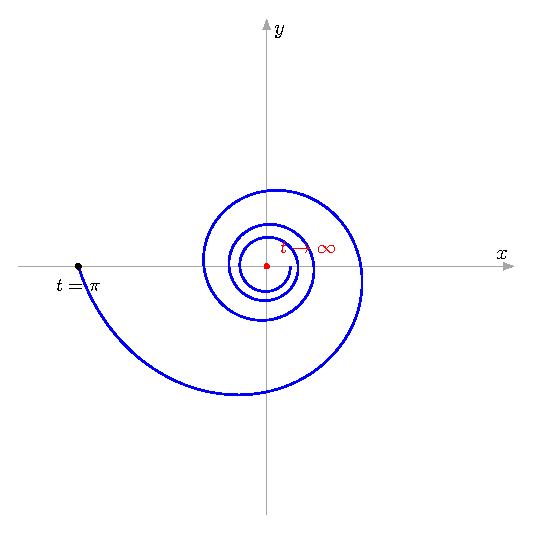
\includegraphics[width=0.4\textwidth]{ej2_1_espiral_decae.pdf}
    \end{figure}
    \item Hacemos ver que
    \begin{align*}
        \gamma'(t)=0 &\implies \left(\left(\cos(t)+\frac{\pi\cos(t)}{t}\right)',\left(\sin(t)+\frac{\pi\sin(t)}{t}\right)'\right)=\left(0,0\right) \\
        &\implies \left(-\sin(t)+\frac{-\pi\cos(t)-\pi t\sin(t)}{t^2},\cos(t)+\frac{-\pi\sin(t)+\pi t\cos(t)}{t^2}\right)=\left(0,0\right) \\
        &\implies \left(\frac{-t^2\sin(t)-\pi\cos(t)-\pi t\sin(t)}{t^2},\frac{t^2\cos(t)-\pi\sin(t)+\pi t\cos(t)}{t^2}\right)=\left(0,0\right) \\
        &\implies -t^2\sin(t)-\pi\cos(t)-\pi t\sin(t)=0, \quad t^2\cos(t)-\pi\sin(t)+\pi t\cos(t)=0 \\
        &\implies \sin(t)(t^2+\pi t)=-\pi\cos(t), \quad \cos(t)(t^2+\pi t)=\pi\sin(t) \\
        &\implies \frac{\sin(t)(t^2+\pi t)^2}{-\pi}=\pi\sin(t) \\
        &\implies \sin(t)(t^2+\pi t)^2=-\pi^2\sin(t) \\
        &\implies \sin(t)((t^2+\pi t)^2+\pi^2)=0,
    \end{align*}
    de loque se sigue, $\sin(t)=0$. Luego, $\cos(t)\neq 0$, y en adición $\sin(t)(t^2+\pi t)=-\pi\cos(t)$ no tiene solución, de lo que se sigue, $\gamma'(t)\neq (0,0)$ para toda $t\in (\pi,\infty)$. Así, $\Gamma$
    es regular. Respecto a la gráfica, es similar a la del inciso (a), puesto que las coordenadas tanto en $x$ como en $y$ van tomando valores cada vez más pequeños, con la peculiaridad de que los puntos cumplen estar
    fuera de la circunferencia de radio 1 con centro en el origen. Así, nuestra gráfica es la de una espiral que se va enrrollando alrededor de la circunferencia antes mencionada sin tocarla.
    \begin{figure}[H]
        \centering
        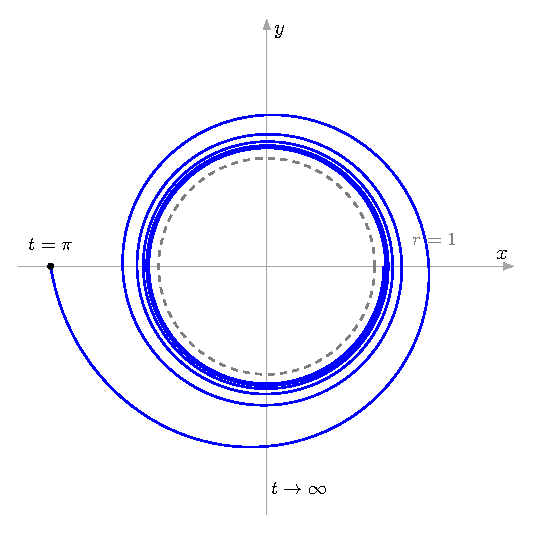
\includegraphics[width=0.4\textwidth]{ej2_2_espiral_asintota.pdf}
    \end{figure}
    \hfill $\blacktriangle$
\end{enumerate}

\newpage
\item Determina una parametrización de las siguientes curvas y muestra si son regulares. Bosqueja la gráfica:
\begin{enumerate}[(1)]
\item La curva descrita por la intersección de $x=z^3$ y $y=1-x$. 
\item La curva dada por la intersección de $x^2+y^2=1$ y $y^2+z^2=1$ con 
$y\neq \pm 1$. 
\end{enumerate}
\textbf{Solución.}
\begin{enumerate}[(i)]
    \item Dado que la función cúbica es biyectiva, aseveramos que $x=z^3$ si y solo si $z=\sqrt[3]{x}$. Puesto que $y=1-x$, de lo dicho anteriormente, obtenemos la parametrización
    \[
    \gamma(t)=\left(t,1-t,\sqrt[3]{t}\right).
    \]
    Dado que la derivada de la primer componente de $\gamma$ es 1, se sigue que $\gamma'(t)\neq (0,0,0)$ para toda $t\in \R$, con lo que afirmamos, la curva previamente descrita es regular.
    \begin{figure}[H]
        \centering
        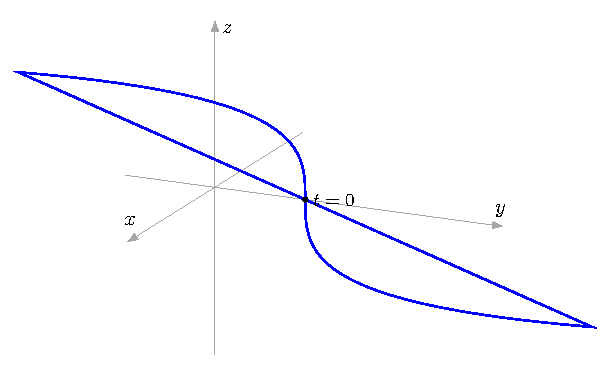
\includegraphics[width=0.4\textwidth]{ej3_1_interseccion_cubica.pdf}
    \end{figure}
    \item De ambas ecuaciones se sigue que
    \begin{align*}
        y^2=1-x^2, \quad y^2=1-z^2 &\iff 1-x^2=1-z^2 \\
        &\iff x^2=z^2 \\
        &\iff (x-z)(x+z)=0 \\
        &\iff z=x, \quad \text{o } z=-x. \tag{1}
    \end{align*}
    Por otra parte, notemos que el cilindro generado por la ecuación $x^2+y^2=1$ tiene la parametrización
    \[
    \gamma(t,z)=(\cos(t),\sin(t),z).
    \]
    De lo dicho en (1), se sigue que existen dos ecuaciones paramétricas de la intersección deseada y son:
    \[
    \gamma_1(t)=(\cos(t),\sin(t),\cos(t)), \quad \gamma_2(t)=(\cos(t),\sin(t),-\cos(t)),\quad t\neq \pi/2,-\pi/2.
    \]
    Así,
    \[
    \gamma_1'(t)=\left(-\sin(t),\cos(t),-\sin(t)\right), \quad \gamma_2'(t)=\left(-\sin(t),\cos(t),\sin(t)\right).
    \]
    Dado que $\sin(t)$ y $\cos(t)$ no se pueden anular simultáneamente, para las dos parametrizaciones anteriores, se cumple que su derivada
    es distinta de $(0,0,0)$ y por lo tanto son regulares. Señalamos que las gráficas de dichas funciones son circunferencias de radio 1 con centro en el origen vistas desde el plano
    $\Pi_{YZ}$, y desde el plano $\Pi_{XZ}$ son los segmentos de de las rectas $z=x, z=-x$ que van desde $x=-\sqrt{2}/2$ a $x=\sqrt{2}/2$.
    \begin{figure}[H]
        \centering
        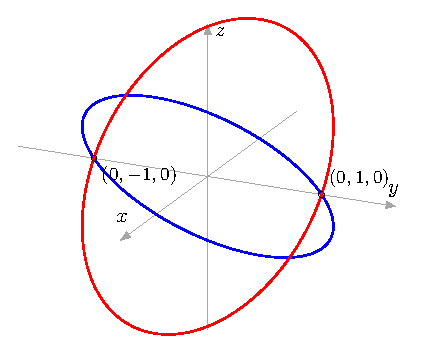
\includegraphics[width=0.4\textwidth]{ej3_2_interseccion_cilindros.pdf}
    \end{figure}
\end{enumerate}
\hfill $\blacktriangle$
\item Demuestra que las líneas tangentes a la curva imagen de 
$\gamma(t)=(\frac{2}{3}t,t^2,t^3)$ forman un ángulo constante con el vector $(1,0,1)$. \\
\textbf{Solución.} A priori tenemos que
\begin{align*}
    \gamma'(t)=\left(\frac{2}{3},2t,3t^2\right).
\end{align*}
Luego, tomemos $t\in \R$ arbitrario. Sabemos que el coseno del ángulo formado por la recta y el vector $(1,0,1)$ es
\begin{align*}
    \cos(\alpha) &= \frac{\left|\left(\frac{2}{3},2t,3t^2\right)\cdot (1,0,1)\right|}{\norm{\left(\frac{2}{3},2t,3t^2\right)}\norm{(1,0,1)}} \\
    &= \frac{\abs{\frac{2}{3}+3t^2}}{\sqrt{\left(\frac{2}{3}\right)^2+4t^2+\left(3t^2\right)^2}\sqrt{2}} \\
    &= \frac{\abs{\frac{2}{3}+3t^2}}{\sqrt{\left(\frac{2}{3}+3t^2\right)^2}\sqrt{2}} \\
    &= \frac{\abs{\frac{2}{3}+3t^2}}{\abs{\frac{2}{3}+3t^2}\sqrt{2}} \\
    &= \frac{\sqrt{2}}{2}.
\end{align*}
De ello, se sigue que $\alpha=\pi/4$, y dado que $t$ fue arbitario, lo anterior se cumple para toda $t$, concluyendo así que el ángulo es constante. \hfill $\blacktriangle$

\newpage
\item Muestra que la curva descrita por la aplicaci\'on 
\[ \gamma(t) = (\sen(2t),2\sen^2(t),2\cos(t)),\qquad (t\in \R) \] 
est\'a contenida en una esfera con centro en el origen. Calcula su rapidez y muestra que la proyecci\'on de su velocidad en el plano $xy$ tiene norma constante. \\
\textbf{Demostración.} Primero hacemos ver que
\begin{align*}
    \norm{\gamma(t)} &= \sqrt{\sin^2(2t)+4\sin^4(t)+4\cos^2(t)} \\
    &= \sqrt{4\sin^2(t)\cos^2(t)+4\sin^4(t)+4\cos^2(t)} \\
    &= \sqrt{4\sin^2(t)(\cos^2(t)+\sin^2(t))+4\cos^2(t)} \\
    &= \sqrt{4(\sin^2(t)+\cos^2(t))} \\
    &= 2.
\end{align*}
Así, afirmamos que todo punto en la curva está contenido en la esfera con centro en el origen de radio 2.
Para calcular la rápidez, hemos de calcular la norma de la derivada. Esto es
\begin{align*}
    \norm{\gamma'(t)} &= \norm{\left(2\cos(2t),4\sin(t)\cos(t),-2\sin(t)\right)} \\
    &= \norm{\left(2\left(\cos^2(t)-\sin^2(t)\right),4\sin(t)\cos(t),-2\sin(t)\right)} \\
    &= \sqrt{4\left(\cos^4(t)-2\cos^2(t)\sin^2(t)+\sin^4(t)\right)+16\sin^2(t)\cos^2(t)+4\sin^2(t)} \\
    &= \sqrt{4\cos^4(t)+8\cos^2(t)\sin^2(t) + 4\sin^4(t) + 4\sin^2(t)} \\
    &= 2\sqrt{\cos^4(t)+2\sin^2(t)\cos^2(t)+\sin^4(t)+\sin^2(t)} \\
    &= 2\sqrt{\cos^2(t)\left(\cos^2(t)+\sin^2(t)\right)+\sin^2(t)(\sin^2(t)+\cos^2(t))+\sin^2(t)} \\
    &= 2\sqrt{1+\sin^2(t)}.
\end{align*}
Por último, notemos que
\begin{align*}
    \norm{P_{XY}\left(\gamma'(t)\right)} &= \norm{\left(2\cos(2t),4\sin(t)\cos(t),0\right)} \\
    &= \norm{\left(2\left(\cos^2(t)-\sin^2(t)\right),4\sin(t)\cos(t),0\right)} \\
    &= \sqrt{4\cos^4(t)+8\cos^2(t)\sin^2(t)+4\sin^4(t)} \\
    &= 2\sqrt{\cos^4(t)+2\cos^2(t)\sin^2(t)+\sin^4(t)} \\
    &= 2\sqrt{\cos^2(t)\left(\cos^2(t)+\sin^2(t)\right)+\sin^2(t)\left(\sin^2(t)+\cos^2(t)\right)} \\
    &= 2\sqrt{\cos^2(t)+\sin^2(t)} \\
    &= 2,
\end{align*}
con lo que concluimos, la proyección de la velocidad de $\gamma(t)$ en el plano $xy$ es de norma constante. \hfill $\blacktriangle$


\newpage
\item Verifica que las siguientes aplicaciones muestran que no se satisface el \emph{teorema del valor medio} para aplicaciones $\gamma:I\subset \R\To \R^m$ e interpreta geom\'etricamente:
\begin{enumerate}[(1)]
\item $\gamma:[-1,1]\To \R^2$ dada por
$$
\gamma(t) = 
\begin{cases}
(-t^2,t^2) & \text{ si } -1\leq t\leq 0, \\
(t^2,t^2) & \text{ si } 0\leq t\leq 1.
\end{cases}
$$
\item $\gamma:[0,1]\To \R^3$ dada por $\gamma(t)=(\cos(2\pi t),\sen(2\pi t),t)$.
\end{enumerate}
\textbf{Solución.}
\begin{enumerate}
    \item Notemos que
    \[
        \gamma'(t) = 
        \begin{cases}
            (-2t,2t) & \text{ si } -1\leq t\leq 0, \\
            (2t,2t) & \text{ si } 0\leq t\leq 1.
        \end{cases}
    \]
    Luego,
    \[
    \frac{\gamma(1)-\gamma(-1)}{1-(-1)} = \frac{(1,1)-(-1,1)}{2} = (1,0). \tag{1}
    \]
    Dada la definición de $\gamma'(t)$, afirmamos que si una de las coordanadas de la derivada es 0, la derivada es el punto $(0,0)$,
    con lo que afirmamos, no es posibles obtener $(1)$, y en consecuencia, no puede cumplirse el teorema del valor medio. Geométricamente, esto se debe a que presenta cierto pico en el $(0,0)$,
    de lo que se deduce, la función no es continua en todo $[-1,1]$.
    \item Hacemos ver que
    \[
    \gamma'(t)=(-2\pi\sin(2\pi t),2\pi\cos(2\pi t),1).
    \]
    Por otra parte,
    \begin{align*}
        \frac{\gamma(1)-\gamma(0)}{1-0} &= (\cos(2\pi),\sen(2\pi),1) - (\cos(0),\sen(0),0) \\
        &= (1,0,1)-(1,0,0) \\
        &= (0,0,1).
    \end{align*}
    Luego, supongamos que existe $c$ tal que se cumple la siguiente igualdad
    \begin{align*}
        \gamma'(c)=(0,0,1) &\iff (-2\pi\sin(2\pi c),2\pi\cos(2\pi c),1)=(0,0,1) \\
        &\iff -2\pi\sin(2\pi c)=0, \quad 2\pi\cos(2\pi c)=0 \\
        &\iff \sin(2\pi c)=0, \quad \cos(2\pi c)=0,
    \end{align*}
    lo cual no es posible puesto que $\cos(x)$ y $\sin(x)$ no pueden anularse en el mismo punto, de lo que se argüye, no existe tal $c$, y por tanto
    no se cumple el teorema del valor medio. Geométricamente, se debe que al tratarse de una función periódica, los puntos de $\gamma(t)$ en 0 y en 1, son los mismos,
    y por lo tanto la recta generada por los punto $\gamma(0),\gamma(1)$ no existe. \hfill $\blacktriangle$
\end{enumerate}

\end{enumerate}

\end{document}
